% !TEX TS-program = xelatex
% !TEX encoding = UTF-8
% !Mode:: "TeX:UTF-8"

\documentclass[onecolumn,oneside]{SUSTechHomework}

\usepackage{blindtext}
\usepackage{graphicx}
\usepackage{subfigure}
\usepackage{float}
\usepackage{listings}
\usepackage{hyperref}
\usepackage{framed}
\usepackage{extarrows}
\usepackage{algorithm}
\usepackage{algorithmic}
\hypersetup{hidelinks,
	colorlinks=true,
	allcolors=black,
	pdfstartview=Fit,
	breaklinks=true}

\begin{document}

% title 
% =====================================================================
\title{Lab 6: z-transform and LTI system in Transformed Domain}
\sid{11812214}
\coursecode{EE323}
\coursename{Digital Signal Processing}
\author{任振裕}
\date{December 2, 2020}
\maketitle 
% Contents
\tableofcontents
% introduction
% =====================================================================
\section*{6.1 Introduction}
\addcontentsline{toc}{section}{6.1 Introduction}
There are mainly two parts of this lab: 
\begin{itemize}
    \item \textbf{z-transform:}\\
    The z-transform is useful for the manipulation of discrete data sequences and has 
    acquired a new significance in the formulation and analysis of discrete-time 
    systems. And in this part of the lab, we will both discuss z-transform and inverse 
    z-transform deeply through many aspects: ROC regions, poles, zeros etc. We will also discuss
    a special case of z-transform that $z=e^{j\omega}$ to calculate the frequency response of a LTI
    system. Through this part, we could have a deeper understanding towards z-transform and LTI system. And this
    will help us a lot for the further filter design.
    \item \textbf{LTI system in Transformed Domain:}\\
    In this part, we will mainly consider two digital filters: Linear phase FIR filters and IIR filters. Linear Phase FIR filters are an important class of FIR filters.
    We will use four basic types of it to have a further exploration for it. In the part of IIR filter, we will involve a simple first order filter.
    All these could help us have a first insight into the digital filter designs.
\end{itemize}
\section*{6.2 z-transform}
\addcontentsline{toc}{section}{6.2 z-transform}
\subsection*{6.2.2 Poles and zeros of z-transform}
\addcontentsline{toc}{subsection}{6.2.2 Poles and zeros of z-transform}
\begin{itemize}
    \item Three functions considered in this section:
    $$
    \begin{aligned}
        H_{1}(z)&=-1+2 z^{-1}-3 z^{-2}+6 z^{-3}-3 z^{-4}+2 z^{-5}-z^{-6} \\
        G_{1}(z)&=\frac{3 z^{4}-2.4 z^{3}+15.36 z^{2}+3.84 z+9}{5 z^{4}-8.5 z^{3}+17.6 z^{2}+4.7 z-6} \\
        G_{2}(z)&=\frac{2 z^{4}+0.2 z^{3}+6.4 z^{2}+4.6 z+2.4}{5 z^{4}+z^{3}+6.6 z^{2}+4.2 z+24}
    \end{aligned}
    $$
    \item MATLAB codes for this section:
\end{itemize}
\begin{lstlisting}[title=\textbf{q6\_2\_2.m}]
    clear;
    P1 = [-1 2 -3 6 -3 2 -1];
    D1 = [1 zeros(1,6)];
    P2 = [3 -2.4 15.36 3.84 9];
    D2 = [5 -8.5 17.6 4.7 -6];
    P3 = [2 0.2 6.4 4.6 2.4];
    D3 = [5 1 6.6 4.2 24];
    zeros1 = roots(P1);poles1 = roots(D1);display(zeros1);display(poles1);
    zeros2 = roots(P2);poles2 = roots(D2);display(zeros2);display(poles2);
    zeros3 = roots(P3);poles3 = roots(D3);display(zeros3);display(poles3);
    subplot(131),zplane(zeros1,poles1),title('H_1(z)');
    subplot(132),zplane(zeros2,poles2),title('G_1(z)');
    subplot(133),zplane(zeros3,poles3),title('G_2(z)');
\end{lstlisting}
\begin{itemize}
    \item Zero-Pole plots:
    \begin{figure}[H]
        \centering
        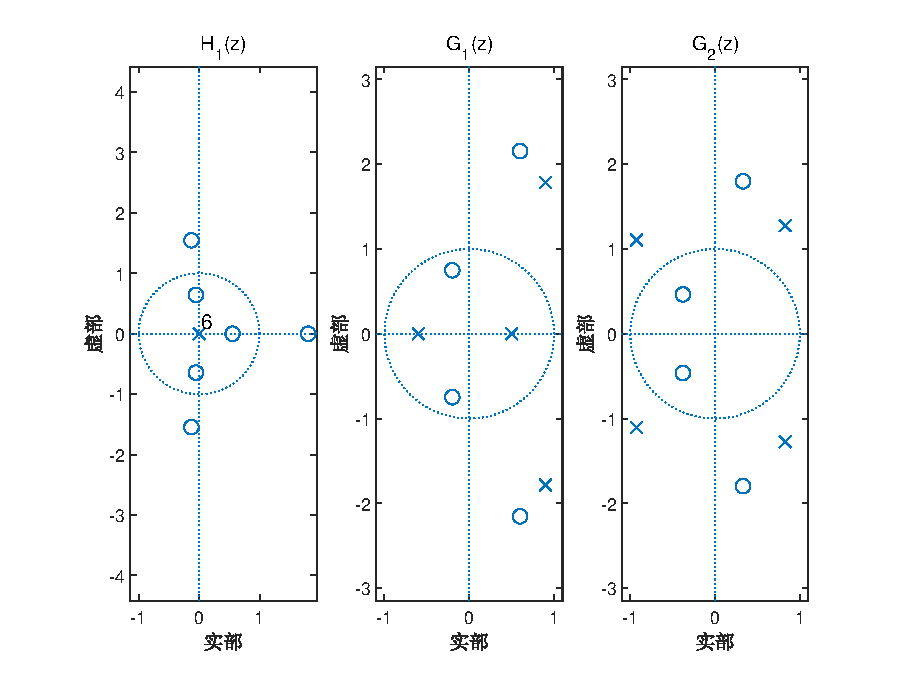
\includegraphics[width=140mm]{pictures/q6_2_2.eps}
        \caption{Zero-Pole plots}
    \end{figure}
    \begin{info}
        To decide the possible ROC region, we used the rules below:
        \begin{itemize}
            \item For right-sided sequences: ROC extends outward from the outermost pole to infinity.
            \item For left-sided: ROC inwards from the innermost pole to the original point.
            \item For two-sided: ROC either is a ring or do not exist.
        \end{itemize}
    \end{info}
    \item For $H_1(z)$:
    \begin{itemize}
        \item Poles: 0, 0, 0, 0, 0, 0 (Or a $6^{\text{th}}$ pole at zero).
        \item Zeros: 1.8054 + 0.0000i, -0.1269 + 1.5457i, -0.1269 - 1.5457i, -0.0528 + 0.6426i, -0.0528 - 0.6426i, 0.5539 + 0.0000i.
        \item Possible ROC:
        \begin{itemize}
            \item left-sided: Impossible since poles are all zero.
            \item right-sided: $\text{ROC}=\left\{z:|z|>0\right\}=\left\{-\infty,0\right\}\cup\left\{0,+\infty\right\} $.
            \item two-sided: Impossible since poles are all zero.
        \end{itemize}
    \end{itemize}
    \item For $G_1(z)$:
    \begin{itemize}
        \item Poles: 0.9000 + 1.7861i, 0.9000 - 1.7861i, -0.6000 + 0.0000i, 0.5000 + 0.0000i.
        \item Zeros: 0.6000 + 2.1541i, 0.6000 - 2.1541i, -0.2000 + 0.7483i, -0.2000 - 0.7483i.
        \item Possible ROC:
        \begin{itemize}
            \item To get the possible ROC, first derive the outermost and innermost poles:
\begin{commandline}
    >> max(abs(poles2))

    ans =
    
        2.0000
    
    >> min(abs(poles2))
    
    ans =
    
        0.5000
\end{commandline}            
            \item left-sided: $\text{ROC}=\left\{z:|z|<0.5\right\}$.
            \item right-sided: $\text{ROC}=\left\{z:|z|>2\right\}$.
            \item two-sided: $\text{ROC}=\left\{z:0.5<|z|<2\right\}$.
        \end{itemize}
    \end{itemize}
    \item For $G_2(z)$:
    \begin{itemize}
        \item Poles: 0.8272 + 1.2744i, 0.8272 - 1.2744i, -0.9272 + 1.1045i, -0.9272 - 1.1045i.
        \item Zeros: 0.3296 + 1.7980i, 0.3296 - 1.7980i, -0.3796 + 0.4637i, -0.3796 - 0.4637i.
        \item Possible ROC:
        \begin{itemize}
            \item To get the possible ROC, first derive the outermost and innermost poles:
\begin{commandline}
    >> max(abs(poles3))

    ans =
    
        1.5193
    
    >> min(abs(poles3))
    
    ans =
    
        1.4421
\end{commandline}
            \item left-sided:  $\text{ROC}=\left\{z:|z|<1.4421\right\}$.
            \item right-sided: $\text{ROC}=\left\{z:|z|>1.5193\right\}$ 
            \item two-sided: $\text{ROC}=\left\{z:1.4421<|z|<1.5193\right\}$.
        \end{itemize}
    \end{itemize}
\end{itemize}

\subsection*{6.2.3 z-transform and frequency response}
\addcontentsline{toc}{subsection}{6.2.3 z-transform and frequency response}
\begin{info}
    For this section, we used the property that $H(e^{j\omega})=\left.H(z)\right|_{|z|=1}$ to plot magnitude and phase response.
\end{info}
\begin{itemize}
    \item Two transfer functions for this section:
    \begin{itemize}
        \item $H(z)=z^{-4}+2 z^{-3}+2 z^{-1}+1$.
        \item $H(z)=\frac{z^{2}-1}{z^{2}-1 \cdot 2 z+0.95}$.
    \end{itemize}
    \item MATLAB function for this section:
\end{itemize}
\begin{lstlisting}[title=\textbf{FreRes.m}]
    function [mag,phase] = FreRes(num,den)
    % num, and den are vectors specifying the coefficients of numerator and denominator.
    % Calculate the function expression and then use fplot to plot it.
    nP = 0:-1:1-length(num);% The index of z for numerator: z^0, z^(-1),z^(-2),...
    nD = 0:-1:1-length(den);% The index of z for denominator: z^0, z^(-1),z^(-2),...
    syms w;
    P = sum(num.*exp(j*w).^nP)% numerator
    D = sum(den.*exp(j*w).^nD)% denonminator
    H = P/D % Obtain the function expression of the transfer function.
    mag = abs(H); phase = angle(H); 
    % sgtitle({'Transfer function: ',char(H)},'FontSize',10)
    subplot(131),fplot(w,(abs(H)),[-pi,pi]);
    xlabel('w(rad)'),ylabel('magnitude response');
    title('magnitude response');
    subplot(132),fplot(w,20*log10(abs(H)),[-pi,pi]);% magnitude in dB
    xlabel('w(rad)'),ylabel('magnitude response(dB)');
    title('magnitude response(dB)');hold on;
    subplot(133),fplot(w,angle(H),[-pi,pi]);% phase
    xlabel('w(rad)'),ylabel('phase response');
    title('phase response');hold on;
    end
\end{lstlisting}
\begin{itemize}
    \item For $H(z)=z^{-4}+2 z^{-3}+2 z^{-1}+1$:
\begin{commandline}
    >> FreRes([1 2 2 1],1)
 
    P =
     
    2*exp(-w*1i) + 2*exp(-w*2i) + exp(-w*3i) + 1
     
     
    D =
     
    1
     
     
    H =
     
    2*exp(-w*1i) + 2*exp(-w*2i) + exp(-w*3i) + 1
\end{commandline}
    Magnitude and phase response:
    \begin{figure}[H]
        \centering
        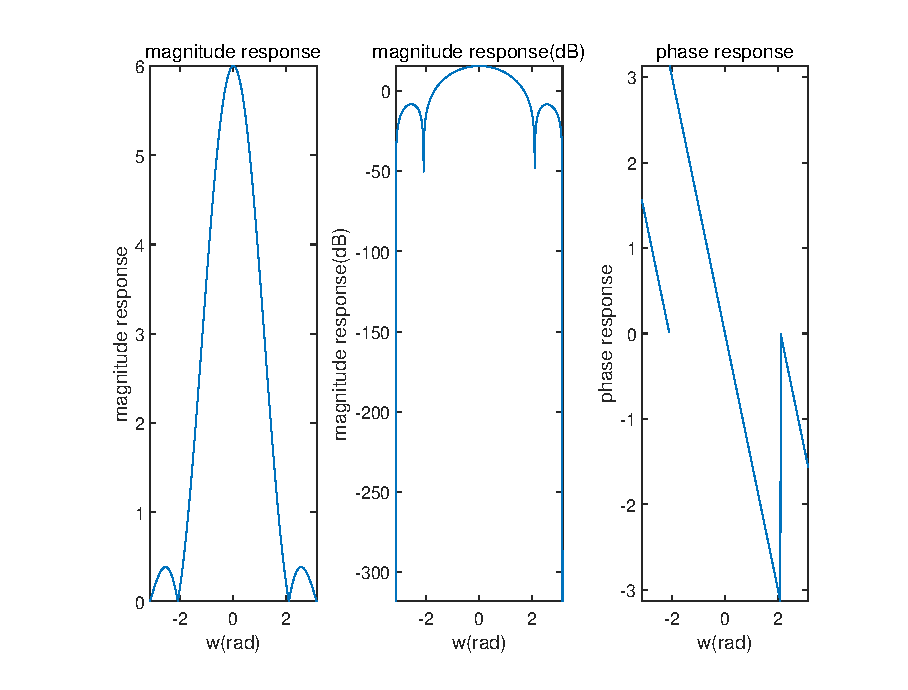
\includegraphics[width=140mm]{pictures/q6_2_3(a).eps}
        \caption{ Magnitude and phase response for $H(z)=z^{-4}+2 z^{-3}+2 z^{-1}+1$}
    \end{figure}
    \item For $H(z)=\frac{z^{2}-1}{z^{2}-1 \cdot 2 z+0.95}=\frac{1-z^{-2}}{1-1.2z^{-1}+0.95z^{-2}}$:
\begin{commandline}
    >> FreRes([1 0 -1],[1 -1.2 0.95])
 
    P =
     
    1 - exp(-w*2i)
     
     
    D =
     
    1 + (19*exp(-w*2i))/20 - (6*exp(-w*1i))/5
     
     
    H =
     
    -(exp(-w*2i) - 1)/(1 + (19*exp(-w*2i))/20 - (6*exp(-w*1i))/5)
\end{commandline}
    Magnitude and phase response:
    \begin{figure}[H]
        \centering
        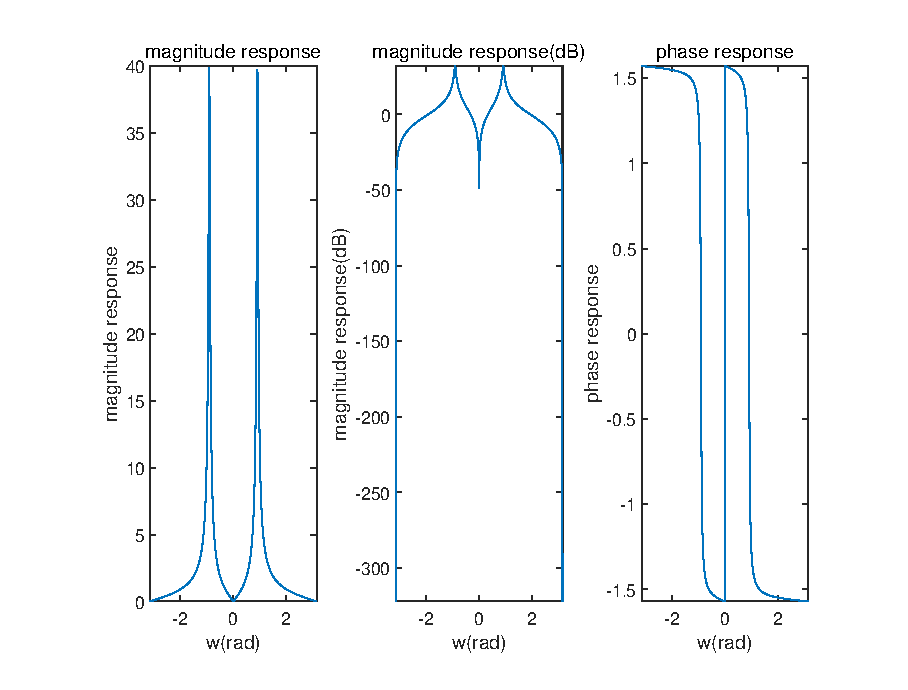
\includegraphics[width=140mm]{pictures/q6_2_3(b).eps}
        \caption{Magnitude and phase response for $H(z)=\frac{z^{2}-1}{z^{2}-1 \cdot 2 z+0.95}$}
    \end{figure}
\end{itemize}
\subsection*{6.2.4 Inverse z-transform}
\addcontentsline{toc}{subsection}{6.2.4 Inverse z-transform}
\begin{itemize}
    \item Two functions considered in this section:
    \begin{itemize}
        \item $X(z)=\frac{3-7.8 z^{-1}}{\left(1-0.7 z^{-1}\right)\left(1+1.6 z^{-1}\right)}$.
        \item $Y(z)=\frac{3 z^{2}+1.8 z+1.28}{(z-0.5)(z+0.4)}$.
    \end{itemize}
    \item The MATLAB function I designed to calculate the partial fraction form:
\end{itemize}
\begin{lstlisting}[title = \textbf{PartialFrac.m}]
    function [rho,lambda,k] = PartialFrac(b,a)
    % input b=[bm ... b1 b0] refers to coefficients of [z^(-m) ... z^(-1) z^0].
    % input a=[an ... a1 a0] refers to coefficients of [z^(-m) ... z^(-1) z^0].
    % b for numerator and a for denominator;
    % Partial fraction format: K(z) + sum(rho/(1-lambda*z^(-1)));
    [r, p, k] = residue(b,a);
    rho = -r./p;
    lambda = 1./p;
    end
\end{lstlisting}
\begin{info}
\begin{itemize}
    \item The partial fraction expansion of z-transform could be expressed as:
    $$
    X(z)=K(z)+\frac{P_{1}(z)}{D(z)}=K(z)+\sum_{l=1}^{N}\left(\frac{\rho_{l}}{1-\lambda_{l} z^{-1}}\right)
    $$
    \item MATLAB function \textbf{residue.m} gives: [r,p,k] = residue(b,a);    
        $$
        \frac{b(s)}{a(s)}=\frac{b_{m} s^{m}+b_{m-1} s^{m-1}+\ldots+b_{1} s+b_{0}}{a_{n} s^{n}+a_{n-1} s^{n-1}+\ldots+a_{1} s+a_{0}}=\frac{r_{n}}{s-p_{n}}+\ldots+\frac{r_{2}}{s-p_{2}}+\frac{r_{1}}{s-p_{1}}+k(s)
        $$
    \item To simplify the computation, I used below substitutions in my code:
    $$
    \begin{aligned}
        &s = z^{-1}\ (\text{Use}\ z^{-1}\ \text{to be the variable of the polynomials});\\
        &\frac{r_{l}}{s-p_{l}} \rightarrow \left(\frac{\rho_{l}}{1-\lambda_{l} z^{-1}}\right) 
    \end{aligned}
    $$
    \item To calculate the inverse z-transform in this section, we used below commonly used z-transformed pairs:
    \begin{itemize}
        \item $-\alpha^{n}\mu[-n-1] \leftrightarrow \frac{1}{1-\alpha z^{-1}} \quad|z|<|\alpha|$.
        \item $\delta[n-m]\leftrightarrow z^{-m} \quad \text { All } z, \text { except } 0(\text { if } m>0) \text { or } \infty(\text { if } m<0)$.
        \item $\alpha^{n} \mu[n] \leftrightarrow \frac{1}{1-\alpha z^{-1}} \quad|z|>|\alpha|$. 
    \end{itemize}
\end{itemize}
\end{info}
\begin{itemize}
    \item For $X(z)=\frac{3-7.8 z^{-1}}{\left(1-0.7 z^{-1}\right)\left(1+1.6 z^{-1}\right)}$:
    \begin{itemize}
        \item $X(z)=\frac{3-7.8 z^{-1}}{\left(1-0.7 z^{-1}\right)\left(1+1.6 z^{-1}\right)}=\frac{-7.8z^{-1}+3}{-1.12z^{-2}+0.9z^{-1}+1}$.
        \item Type below codes in command window of MATLAB:
        \begin{commandline}
            >> [rho,lambda,k] = PartialFrac([-7.8 3],[-1.12 0.9 1])

            rho =
            
               -2.4783\\
                5.4783
            
            
            lambda =
            
                0.7000\\
               -1.6000
            
            
            k =
            
                 []
        \end{commandline}
        \item The partial expansion of $X(z)$'s z-transform: $X(z)=\frac{-2.4783}{1-0.7z^{-1}}+\frac{5.4783}{1+1.6z^{-1}}$.
        \begin{itemize}
            \item When $\text{ROC}=\left\{z:|z|>1.6\right\}$, then $x[n]$ is a right-sided sequence.\\
             $\therefore$ $x[n]=-2.4783(0.7)^nu[n]+5.4783(-1.6)^nu[n]$.
            \item When $\text{ROC}=\left\{z:|z|<0.7\right\}$, then $x[n]$ is a left-sided sequence.\\
            $\therefore$ $x[n]=2.4783(0.7)^nu[-n-1]-5.4783(-1.6)^nu[-n-1]$.
            \item When $\text{ROC}=\left\{z:0.7<|z|<1.6\right\}$, then $x[n]$ is a two-sided sequence.\\
            $\therefore$ $x[n]=-2.4783(0.7)^nu[n]-5.4783(-1.6)^nu[-n-1]$.
        \end{itemize}
    \end{itemize}
    \item For $Y(z)=\frac{3 z^{2}+1.8 z+1.28}{(z-0.5)(z+0.4)}$:
    \begin{itemize}
        \item $Y(z)=\frac{3 z^{2}+1.8 z+1.28}{(z-0.5)(z+0.4)}=\frac{3 z^{2}+1.8 z+1.28}{z^2-0.1z-0.2}=\frac{1.28z^{-2}+1.8z^{-1}+3}{-0.2z^{-2}-0.1z^{-1}+1}$.
        \item Type below codes in command window of MATLAB:
        \begin{commandline}
            >> [rho,lambda,k] = PartialFrac([1.28 1.8 3],[-0.2 -0.1 1])

            rho =
            
                2.8889\\
                6.5111
            
            
            lambda =
            
               -0.4000\\
                0.5000
            
            
            k =
            
               -6.4000            
        \end{commandline}
        \item The partial expansion of $Y(z)$'s z-transform: $Y(z)=-6.4+\frac{2.8889}{1+0.4z^{-1}}+\frac{6.5111}{1-0.5z^{-1}}$.
        \begin{itemize}
            \item When $\text{ROC}=\left\{z:|z|>0.5\right\}$, then $y[n]$ is a right-sided sequence.\\
            $\therefore$ $y[n]=-6.4\delta[n]+2.8889(-0.4)^nu[n]+6.5111(0.5)^nu[n]$.
            \item When $\text{ROC}=\left\{z:|z|<0.4\right\}$, then $y[n]$ is a left-sided sequence.\\
            $\therefore$ $y[n]=6.4\delta[n]-2.8889(-0.4)^nu[-n-1]+6.5111(0.5)^nu[-n-1]$.
            \item When $\text{ROC}=\left\{z:0.4<|z|<0.5\right\}$, then $y[n]$ is a two-sided sequence.\\
            $\therefore$ $\text{ROC}=6.4\delta[n]+2.8889(-0.4)^nu[n]+6.5111(0.5)^nu[-n-1]$.
        \end{itemize} 
    \end{itemize}
\end{itemize}
\subsection*{6.2.5 Stability Conditions}
\addcontentsline{toc}{subsection}{6.2.5 Stability Conditions}
\begin{itemize}
    \item Two functions used in this section:
    \begin{itemize}
        \item $H_1(z)=\frac{1}{1-1.845 z^{-1}+0.850586 z^{-2}}$.
        \item $H_2(z)=\frac{1}{1-1.85 z^{-1}+0.85 z^{-2}}$(The system is implemented by keeping 2 digits after
        the decimal points of the coefficients.).
    \end{itemize}
    \item MATLAB codes for this section:
\end{itemize}
\begin{lstlisting}[title=\textbf{q6\_2\_5.m}]
    clear;
    poles1 = [0.943 0.902]; zeros1 = [0 0];
    b1 = [1]; a1 = [1 -1.845 0.850586];
    [h1,t1] = impz(b1,a1);
    poles2 = [1 0.85]; zeros2 = [0 0];
    b2 = [1]; a2 = [1 -1.85 0.85];
    [h2,t2] = impz(b2,a2);
    figure(1); %H1
    sgtitle('Zero-Pole plot and Impulse Response of H_1(z)')
    subplot(121),zplane(zeros1',poles1'),title('Zero-Pole plot');
    subplot(122),stem(t1,h1),xlabel('t'),ylabel('h'),title('Impulse Response');
    figure(2); %H2
    sgtitle('Zero-Pole plot and Impulse Response of H_2(z)')
    subplot(121),zplane(zeros2',poles2'),title('Zero-Pole plot');
    subplot(122),stem(t2,h2),xlabel('t'),ylabel('h'),title('Impulse Response');     
\end{lstlisting}
\begin{itemize}
    \item For $H_1(z)=\frac{1}{1-1.845 z^{-1}+0.850586 z^{-2}}=\frac{z^2}{z^{2}-1.845 z^{1}+0.850586}$:
    \begin{itemize}
        \item Poles of $H_1(z)$: $z_{p}=\frac{1.845 \pm \sqrt{1.845^{2}-4 \times 0.850586}}{2}=0.943, \text { or } 0.902$.
        \item Roots of $H_1(z)$: 0,0 (Or a $2^{\text{th}}$ root at zero).
        \item Zero-pole plot and impulse response of $H_1(z)$: 
        \begin{figure}[H]
            \centering
            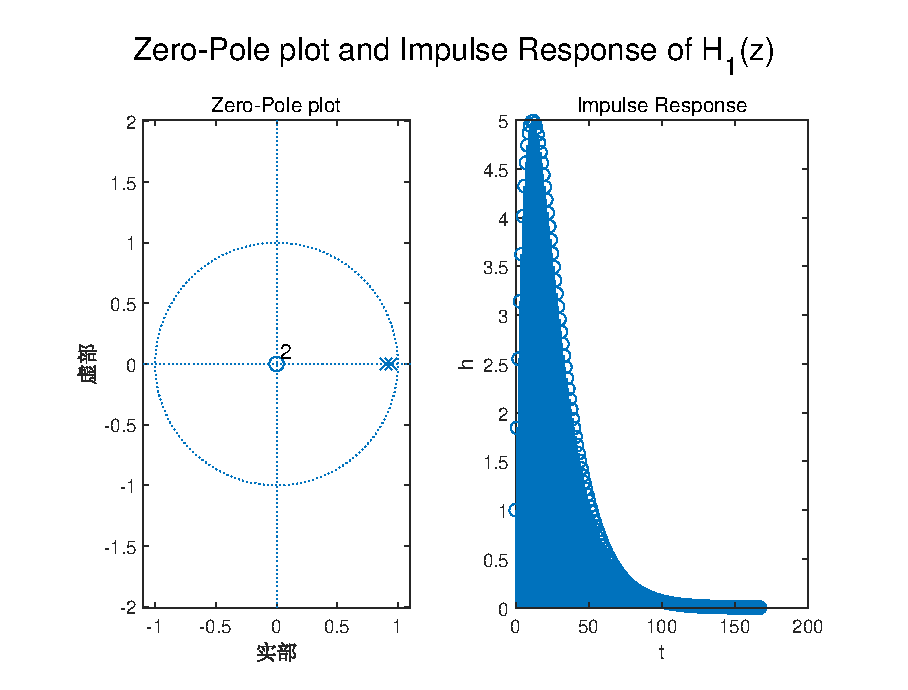
\includegraphics[width=170mm]{pictures/q6_2_5(a).eps}
            \caption{Zero-pole plot and impulse response of $H_1(z)$}
        \end{figure}
    \end{itemize}
    \item For $H_2(z)=\frac{1}{1-1.85 z^{-1}+0.85 z^{-2}}=\frac{z^{2}}{z^{2}-1.85z+0.85}$:
    \begin{itemize}
        \item Poles of $H_2(z)$: $z_{p}=\frac{1.85 \pm \sqrt{1.85^{2}-4 \times 0.85}}{2}=1, \text { or } 0.85$.
        \item Roots of $H_2(z)$: 0,0 (Or a $2^{\text{th}}$ root at zero).
        \item Zero-pole plot and impulse response of $H_2(z)$:
        \begin{figure}[H]
            \centering
            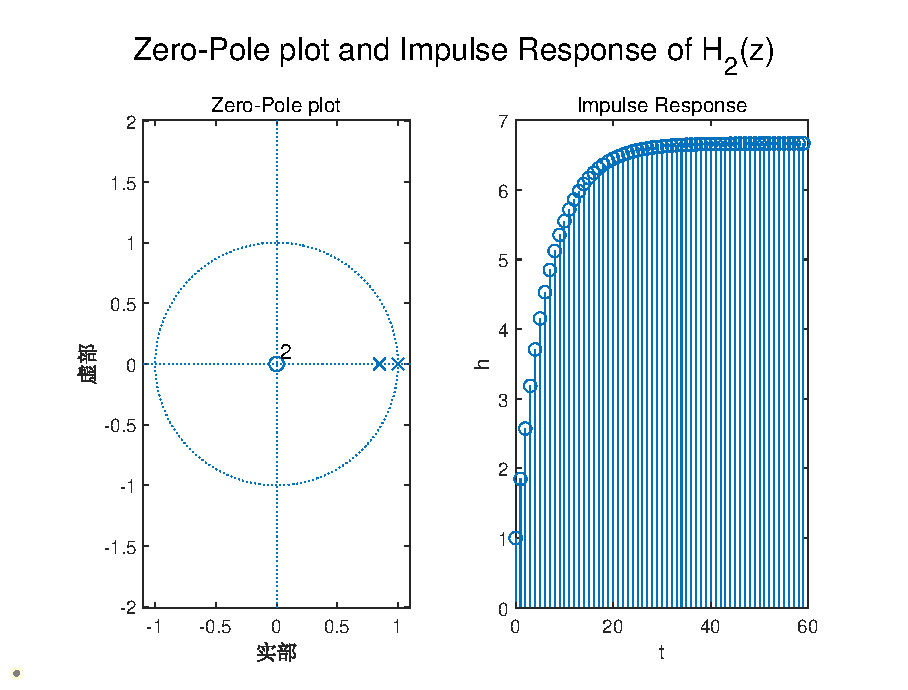
\includegraphics[width=170mm]{pictures/q6_2_5(b).eps}
            \caption{Zero-pole plot and impulse response of $H_2(z)$}
        \end{figure}
    \end{itemize}
    \item Analysis:
    \begin{itemize}
        \item Statistically speaking, magnitudes of poles of $H_1(z)$ are all lower than one while
        those of $H_2(z)$ contain one. This means that $H_1(z)$ is stable while $H_2(z)$ is not stable.
        \item Graphically speaking, according to Figures 3 and 4, all the poles of $H_1(z)$ are within the unit circle while
        one of $H_2(z)$'s poles is on the unit circle, which means that the ROC region of $H_1(z)$ contains the unit circle while
        the ROC region of $H_2(z)$ does not, therefore $H_1(z)$ is stable but $H_2(z)$ is not.
        \item All these changes are caused by ping 2 digits after the decimal pointsof the coefficients.
        This means that an originally stable IIR filter characterized by infinite
        precision coefficients and with all poles inside the unit
        circle may become unstable after implementation due to
        the unavoidable quantization of all coefficients.
    \end{itemize}
\end{itemize}
\section*{6.3 Linear Phase FIR Filters}
\addcontentsline{toc}{section}{6.3 Linear Phase FIR Filters}
\subsection*{6.3.1 Four Types of Linear Phase FIR Filters}
\addcontentsline{toc}{subsection}{6.3.1 Four Types of Linear Phase FIR Filters}
\subsubsection*{A. INLAB report I for section 6.3.1}
\begin{itemize}
    \item Type \MakeUppercase{\romannumeral1} Linear Phase FIR Filter $h[n]$ considered in this section:
    $$
    \begin{aligned}
        \{h[n]\} = \{&-0.0035,-0.0039,0.0072,0.0201,-0.0000,-0.0517,-0.0506,0.0855,0.2965,0.4008 
        \\ & 0.2965,0.0855,-0.0506,-0.0517,-0.0000,0.0201,0.0072,-0.0039,-0.0035\}
         \qquad \text{for}\ 0\leq n \leq 18;  
    \end{aligned}
    $$
    Evidently, $h[n]$ is a symmetric impulse response that satisfies the Type \MakeUppercase{\romannumeral1}, therefore we could get its z-transform in the below format:\\
    $$
    \begin{aligned}
        H(z)=&-0.0035-0.0039z^{-1}+0.0072z^{-2}+0.0201z^{-3}-0.0517z^{-5}-0.0506z^{-6}+0.0855z^{-7}+0.2965z^{-8}\\
             &0.4008z^{-9}+0.2965z^{-10}+0.0855z^{-11} - 0.0506z^{-12}-0.0517z^{-13}+0.0201z^{-15}+0.0072z^{-16}\\ 
             &-0.0039z^{-17} -0.0035z^{-18}
    \end{aligned}
    $$
    \item MATLAB codes in this section:
\end{itemize}
\begin{lstlisting}[title=\textbf{q6\_3\_1a.m}]
    clear;
    h=[-0.0035,-0.0039,0.0072,0.0201,-0.0000,-0.0517,-0.0506,0.0855,0.2965,
    0.4008,0.2965,0.0855,-0.0506,-0.0517,-0.0000,0.0201,0.0072,
    -0.0039,-0.0035]
    figure(1);
    [mag,phase]=FreRes(h,1);
    subplot(132),plot(linspace(-pi,pi,1000),-3*ones(1,1000),'.-')
    figure(2);
    P=h;%Since h is symmetrical impulse response;
    D=[1 zeros(1,18)];
    zeros = roots(P) 
    poles = roots(D)
    zplane(zeros,poles)
\end{lstlisting}
\begin{itemize}
    \item Use \textbf{FreRes.m} to calculate the magnitude and frequency responses:
    \begin{figure}[H]
        \centering
        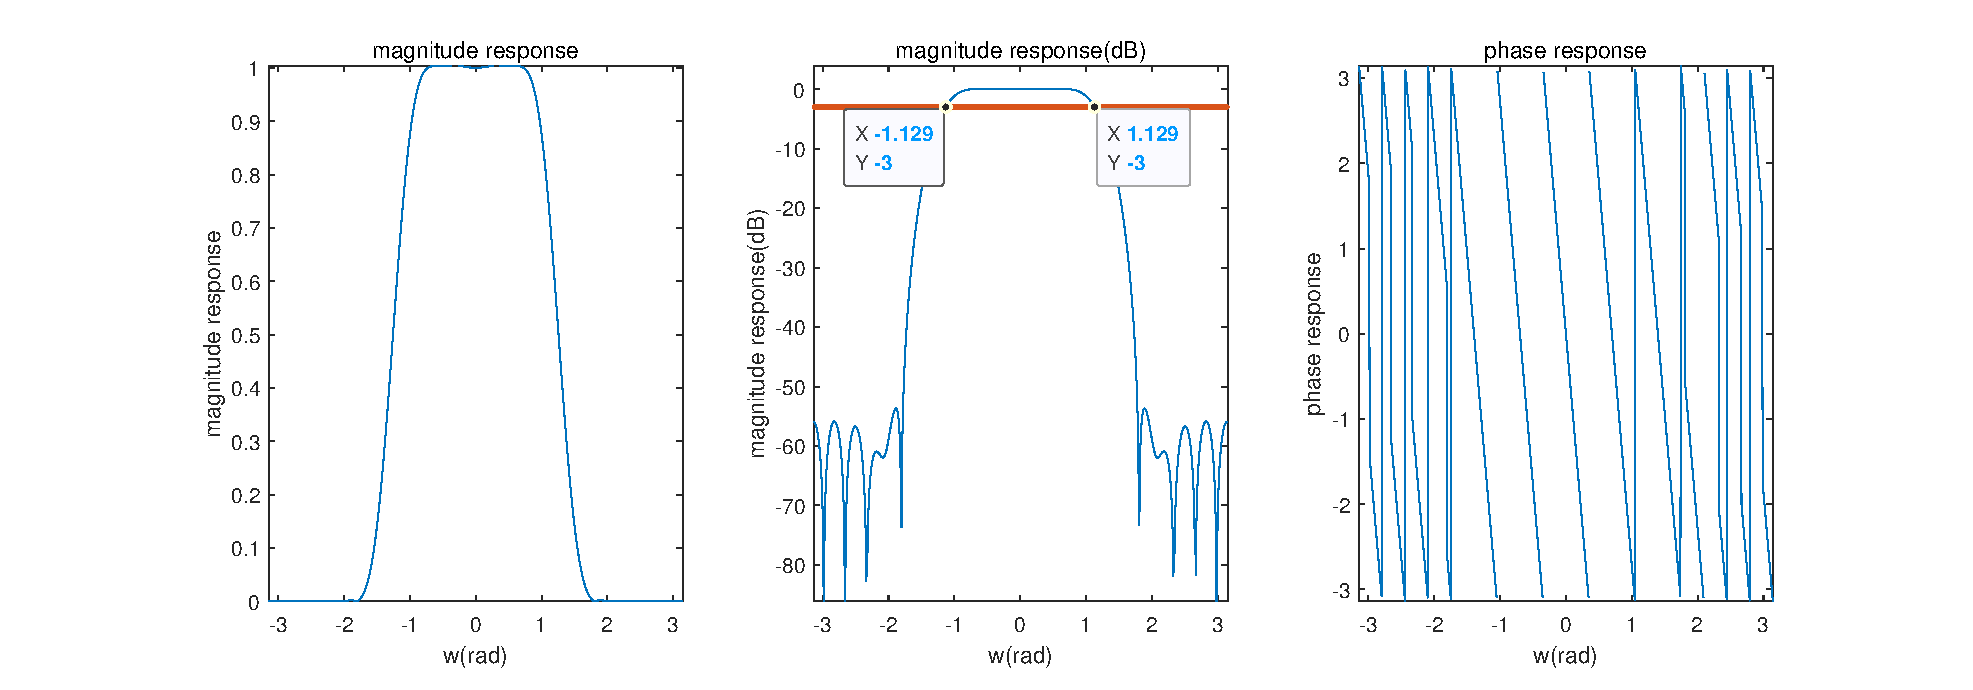
\includegraphics[width=170mm]{pictures/q6_3_1(a).eps}
        \caption{Frequency response of the filter $h[n]$}
    \end{figure}
    \item zero-pole plots of the filter:
    \begin{figure}[H]
        \centering
        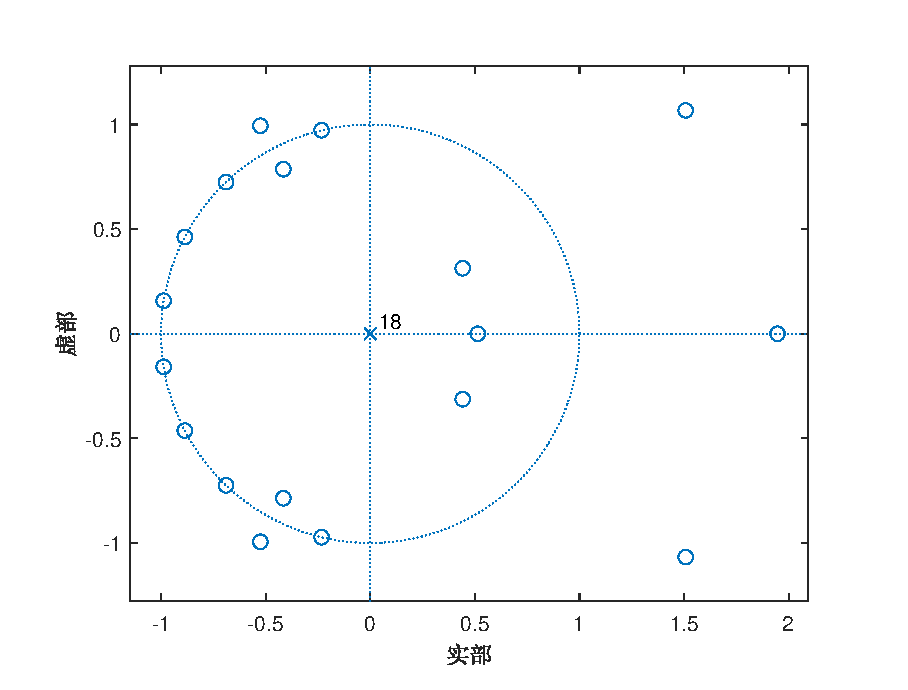
\includegraphics[width=170mm]{pictures/q6_3_1(b).eps}
        \caption{zero-pole plots of the filter}    
    \end{figure}
    \item Analysis for figure 7:\\ 
    The zero-pole plots of figure 7 just suit the property of Type \MakeUppercase{\romannumeral1} Linear Phase FIR filter
    such that Either an even number or no zeros at $z=1$ and $z=-1$ and $H(z)=z^{-(N-1)} H\left(z^{-1}\right)$(Mirror Image Symmetry of Zeros).
    \item Answers to the two questions:
    \begin{itemize}
        \item Question 1 (magnitude characteristic):
        \begin{itemize}
            \item According to Figure 6, $H(e^{j\omega})$ is a lowpass filter but not an ideal filter since the filter 
            not exactly has a magnitude response equal to one in the passband and zero in the stopband, and has a zero phase everywhere. 
            \item And if we use $3$dB cutoff frequency to identify the passband, 
            as shown in the markers of figure, the cutoff frequency $\omega_c$ equals approximately $\pm 1.129$(rad).
            \item The passband of the lowpass filter is $\omega \in [-1.129,1.129]$ in rad with a length $2.258$(rad).
            \item The stopband of the lowpass filter is $\omega \in [-\pi,-1,129]\cup[1.129,\pi]$.
        \end{itemize}
        \item Question 2 (If a type III filter may be designed to be a lowpass filter?):
        \begin{itemize}
            \item Evidently, type III filter can not be designed as a lowpass filter. And I just give a counterexample that just satisfies Anti-symmetrical impulse response with h=[1 -2 3 0 -3 2 -1].
            \item MATLAB code for counterexample:
\begin{lstlisting}[title=\textbf{q6\_3\_1b.m}]
    clear;
    h=[1 -2 3 0 -3 2 -1];
    [mag,phase]=FreRes(h,1);
\end{lstlisting}
        \item Result:
        \begin{figure}[H]
            \centering
            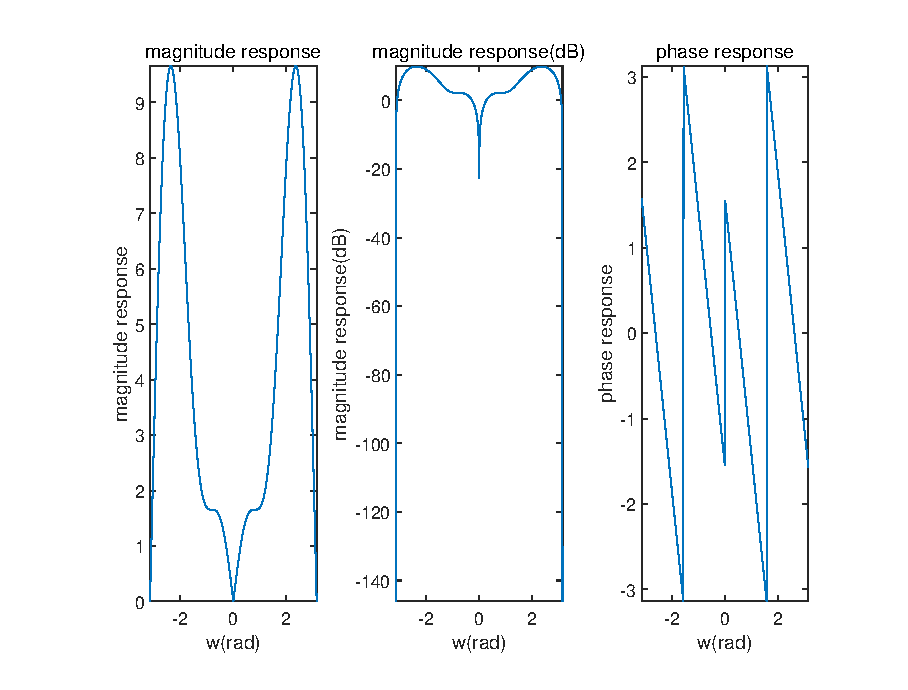
\includegraphics[width=170mm]{pictures/q6_3_1(c).eps}
            \caption{Counterexample for Question 2}
        \end{figure}
        \item Analysis:\\
         According to above figure, the frequency response of Type III can not be a lowpass filter but more like a bandpass filter.
        \end{itemize}
    \end{itemize}
\end{itemize}
\subsubsection*{B. INLAB report II for section 6.3.1}
\begin{itemize}
    \item $h_1[n]$ and $h_2[n]$ considered in this section:
    $$
    \begin{array}{c}h_{1}[n]=\left\{\begin{array}{lr}h[n], & \text { for even } n 
        \\-h[n], & \text { for odd } n\end{array}\right. 
        \\h_{2}[n]=\left\{\begin{array}{lr}h[n / 5], & \text { for } n=5 k \text { for interger } k 
            \\0, & \text { otherwise }\end{array}\right.
    \end{array}
    $$
    \item MATLAB code for this section:
\end{itemize}

\begin{lstlisting}[title=\textbf{q6\_3\_1c.m}]
    clear;
    n=0:18;
    h=[-0.0035,-0.0039,0.0072,0.0201,-0.0000,-0.0517,-0.0506,0.0855,0.2965,
    0.4008,0.2965,0.0855,-0.0506,-0.0517,-0.0000,0.0201,
    0.0072,-0.0039,-0.0035]
    h1=h;h2=zeros(1,91);
    h1(2:2:19)=-h1(2:2:19);
    h2(1:5:91)=h(1:1:19);
    figure(1);% frequency response of h1[n]
    [mag1,phase1]=FreRes(h1,1);
    figure(2);% frequency response of h2[n]
    [mag2,phase2]=FreRes(h2,1);
\end{lstlisting}
\begin{itemize}
    \item Frequency response of $h_1[n]$:
    \begin{figure}[H]
        \centering
        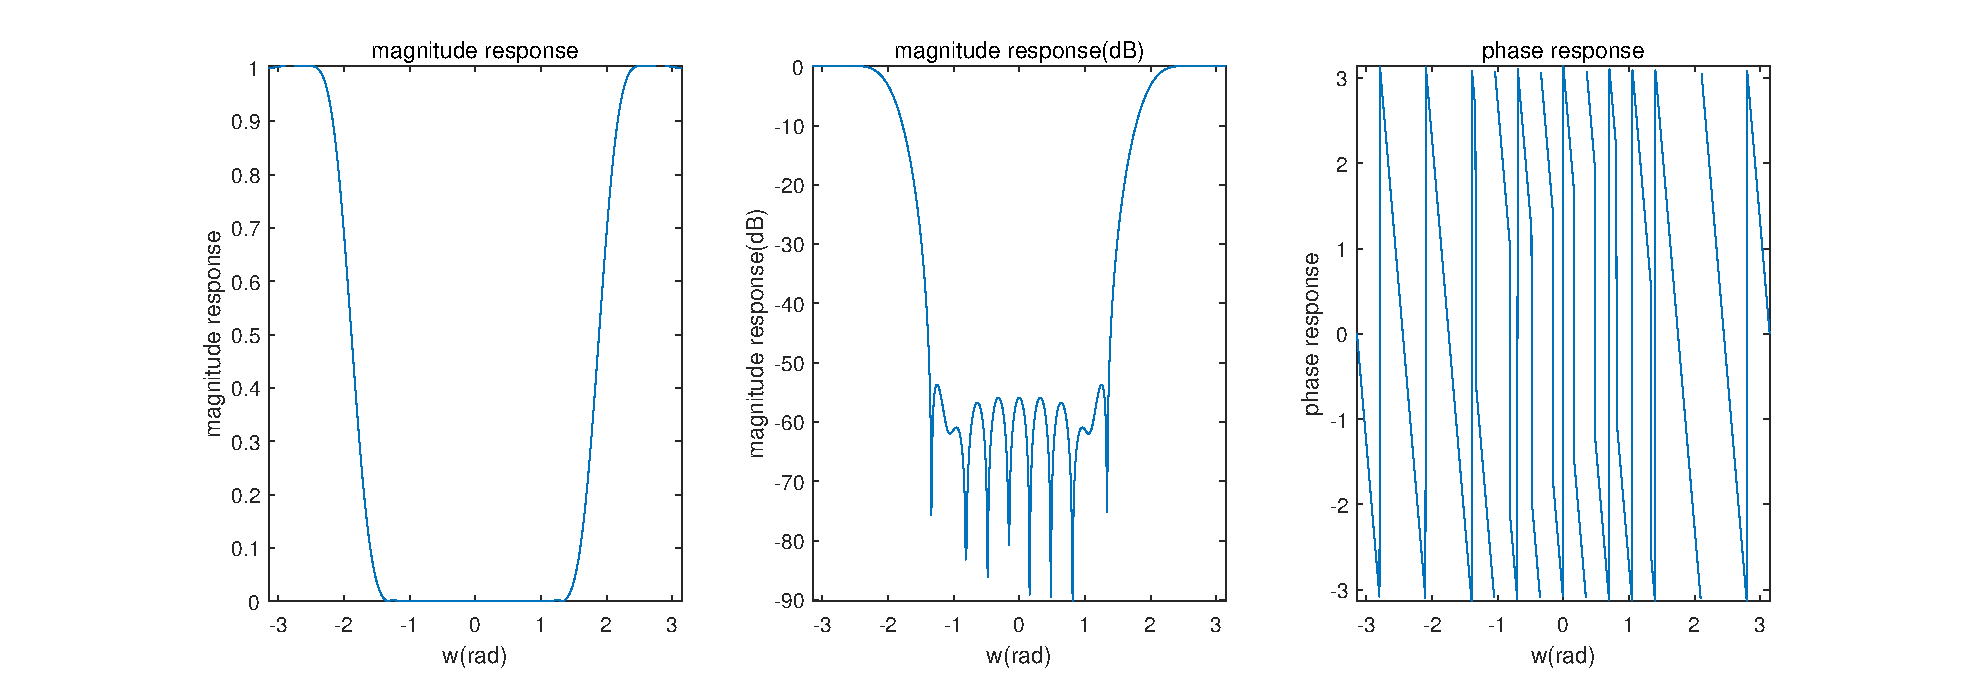
\includegraphics[width=170mm]{pictures/h1_FreRes.eps}
        \caption{Frequency response of $h_1[n]$}
    \end{figure}
    \item Frequency response of $h_2[n]$:
    \begin{figure}[H]
        \centering
        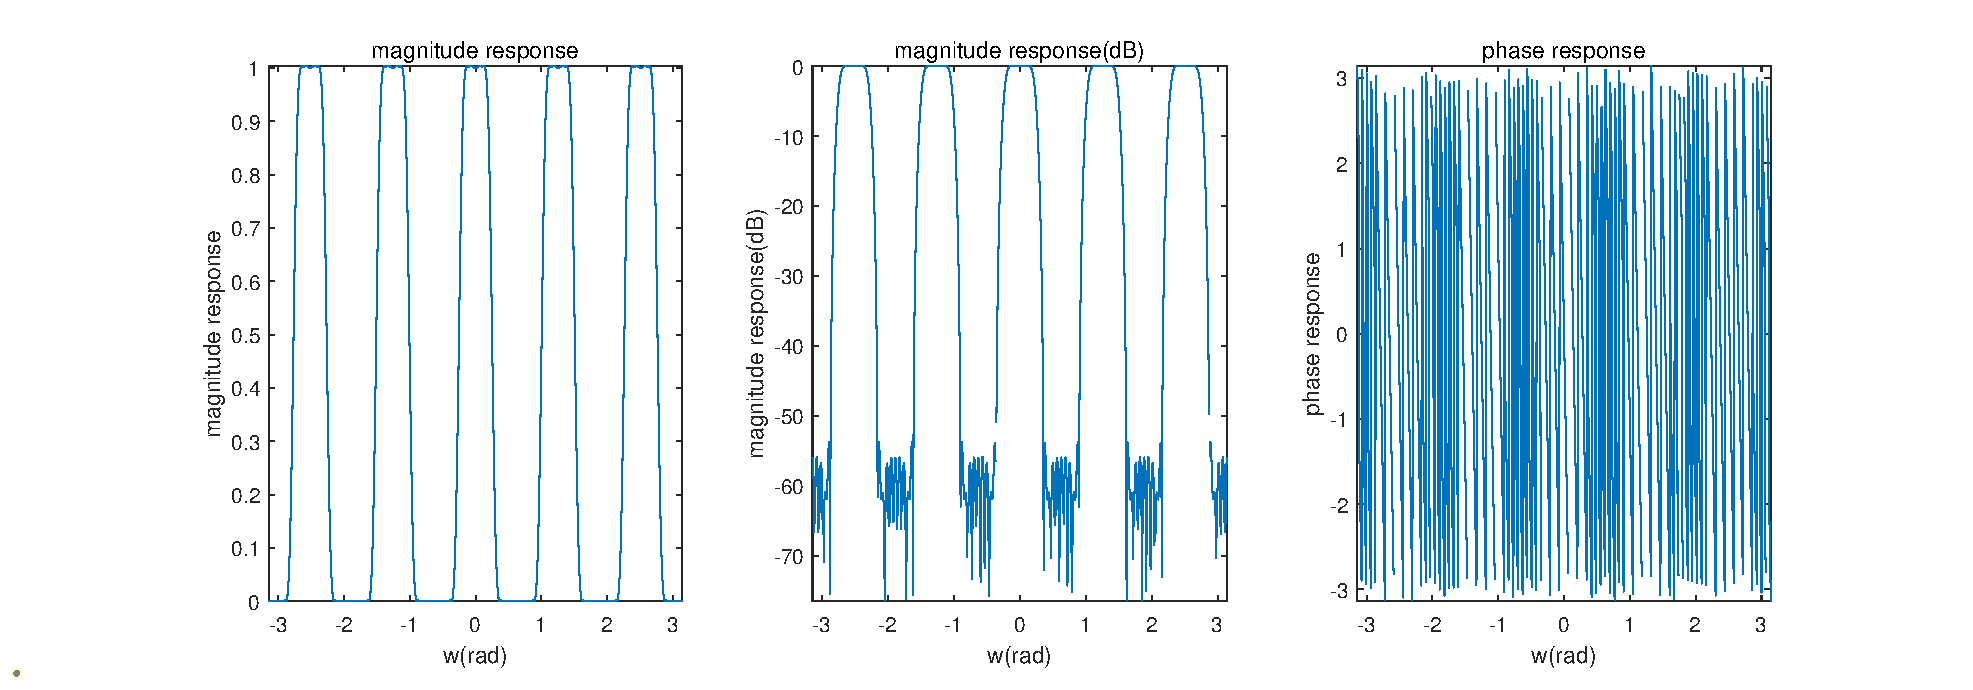
\includegraphics[width=170mm]{pictures/h2_FreRes.eps}
        \caption{Frequency response of $h_2[n]$}
    \end{figure}
    \item Analysis:
    \begin{itemize}
        \item For $h_1[n]$, we firstly derive the relationship of z-transform between $h_1[n]$ and $h[n]$:
        $$
        \begin{aligned}
            H(-z)&=\sum_{n=-\infty}^{\infty} h[n](-z)^{-n}\\
            &=\sum_{n=-\infty}^{\infty} h[n](z)^{-n}(-1)^{-n}\\
            &=\sum_{n=-\infty}^{\infty} h\left[n_{\text {even}}\right](z)^{-n_{\text {even}}}-\sum_{n=-\infty}^{\infty} h\left[n_{\text {odd}}\right](z)^{-n_{\text{odd}}}
            \\ & =H_{1}(z)    
        \end{aligned}
        $$
        $\therefore$ we have $H_1(e^{j\omega})=H(-e^{j\omega})=H(e^{j(\omega+\pi)})$. This will make the frequency response of $H_1(z)$ is a right frequncy shift with $\pi$ of $H(z)$.
        \\ By comparing the frequency responses of Figures 6 and 9, we could verify the above conclusion.
        \item For $h_2[n]$, we have below general property for time-scaling signal:
        \begin{info}
        If $x_{(k)}[n]$ satisfies:
        $$
        x_{(k)}[n]=\left\{\begin{array}{ll}x[n / k], & \text { if } n \text { is a multiple of } k \\0, & \text { if } n \text { is not a multiple of } k\end{array}\right.
        $$
        Then we have:
        $$
        X_{(k)}\left(e^{j \omega}\right)=\sum_{n=-\infty}^{+\infty} x_{(k)}[n] e^{-j \omega n}=\sum_{r=-\infty}^{+\infty} x_{(k)}[r k] e^{-j \omega r k}
        $$
        Furthermore, since $x_{(k)}[r k]=x[r]$, we can find that:
        $$
        X_{(k)}\left(e^{j \omega}\right)=\sum_{r=-\infty}^{+\infty} x[r] e^{-j(k \omega) r}=X\left(e^{j k \omega}\right)
        $$
        Finally, that is:
        $$
        x_{(k)}[n] \stackrel{\mathrm{Ft}}{\longleftrightarrow} X\left(e^{j k \omega}\right)
        $$
        \end{info}
        $\therefore$ For this case, we have $H_2(e^{j\omega})=H(e^{j5\omega})$.\\
        This means that the period of $H_2(e^{j\omega})$ is $1/5$ of $H(e^{j5\omega})$. And if we
        compare the Figrues 6 and 10, we can verify this conclusion.
    \end{itemize}
\end{itemize}
\subsection*{6.3.2 Design of Simple FIR Filters}
\addcontentsline{toc}{subsection}{6.3.2 Design of Simple FIR Filters}
\begin{info}
\begin{itemize}
    \item In this section, we need to design a linear phase lowpass FIR filter with a 3-dB cutoff frequency at $0.3\pi$ using two methods:
    \begin{itemize}
        \item A cascade of first-order lowpass filters.
        \item A higher order moving average filter.
    \end{itemize}
    \item First-order lowpass filter: $H_{0}(z)=\frac{1+z^{-1}}{2}=e^{-j \omega / 2} \cos (\omega / 2)$. \\
    M-order lowpass filter: 
    $$
    \begin{aligned}
        H(z)&=\left(\frac{1+z^{-1}}{2}\right)^M\\
        H(e^{j\omega})&=e^{-j M\omega / 2} \cos ^M(\omega / 2)
    \end{aligned}
    $$ 
\end{itemize}
\end{info}
\begin{info}
    \begin{itemize}
        \item To get the number of stages of the lowpass filter:
        $$
        \text{Solve the equation} \qquad \cos ^M(\omega_c / 2) = \frac{\sqrt{2}}{2}
        $$
        $\therefore$ $\omega_{c}=2 \cos ^{-1}\left(2^{-1 /(2 M)}\right)$.\\
        When $\omega_c=0.3\pi$ $\rightarrow$ $M=3$.
        \item A cascade of first-order lowpass filters: 
        $$
        \begin{aligned}
            H(z)&=\left(\frac{1+z^{-1}}{2}\right)^M=\left(\frac{1+z^{-1}}{2}\right)^3\\
            H(e^{j\omega})&=e^{-j 3\omega / 2} \cos ^3(\omega / 2)\\
        \end{aligned}
        $$
        \item A higher order moving average filter:
        $$
        \begin{aligned}
            H(\mathrm{z})=\frac{1}{M} \sum_{m=0}^{M-1} z^{-m}\ &\xlongrightarrow\ H\left(e^{j \omega}\right)=\frac{1}{M} \cdot \frac{\sin \left(\frac{M \omega}{2}\right)}{\sin \left(\frac{\omega}{2}\right)} e^{-\frac{j(M-1) \omega}{2}}
            \\ H\left(e^{j \omega}\right)
            &=\frac{1}{3} \cdot \frac{\sin \left(\frac{3 \omega}{2}\right)}{\sin \left(\frac{\omega}{2}\right)} e^{-\frac{j2 \omega}{2}}
        \end{aligned}
        $$
    \end{itemize}
\end{info}
\begin{itemize}
    \item MATLAB code for this section:
\end{itemize}
\begin{lstlisting}[title=\textbf{q6\_3\_2.m}]
    clear;
    w = linspace(0,pi,5000);
    M = 3;
    H_cascade = exp(-j*3*w/2).*(cos(w/2)).^3;
    H_moving_average = (1/M)*sin(M.*w/2)./sin(w/2).*exp(-1j*(M-1).*w./2);
    plot(w,10*log10(abs(H_cascade)));
    hold on;
    plot(w,10*log10(abs(H_moving_average)));
    plot(w,-3*ones(1,5000));
    ylim([-50,0]);
    legend('the cascade filter','higher order moving average filter','3-dB cutoff line');
\end{lstlisting}
\begin{itemize}
    \item The plot of two designs and 3dB cutoff frequency:
    \begin{figure}[H]
    \centering
    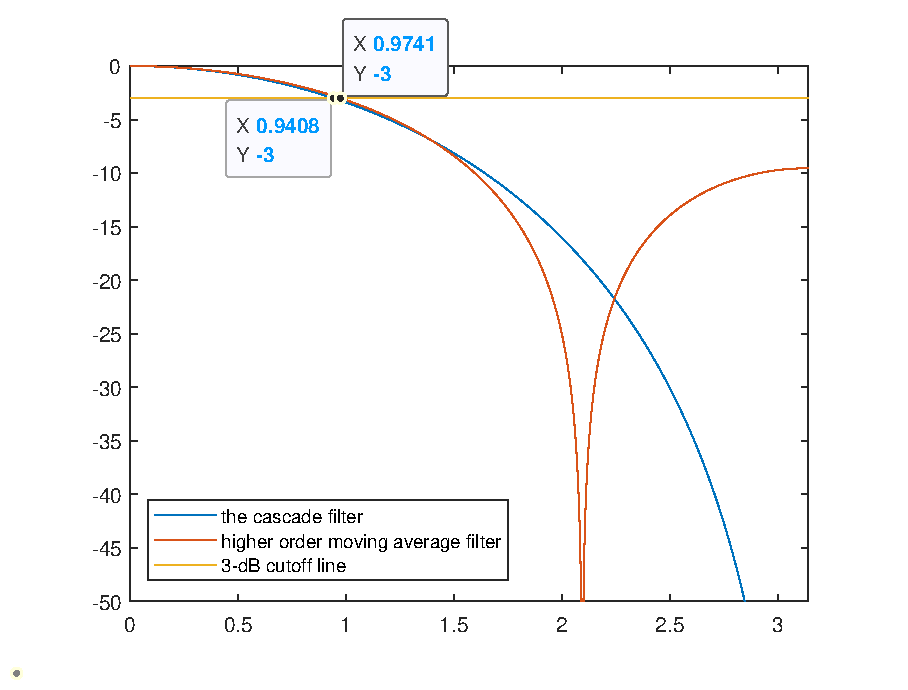
\includegraphics[width=140mm]{pictures/twodesigns1.eps}
    \caption{The plot of two designs and 3dB cutoff frequency}
    \end{figure}
    \item A tiny look for cutoff frequency:
    \begin{figure}[H]
    \centering
    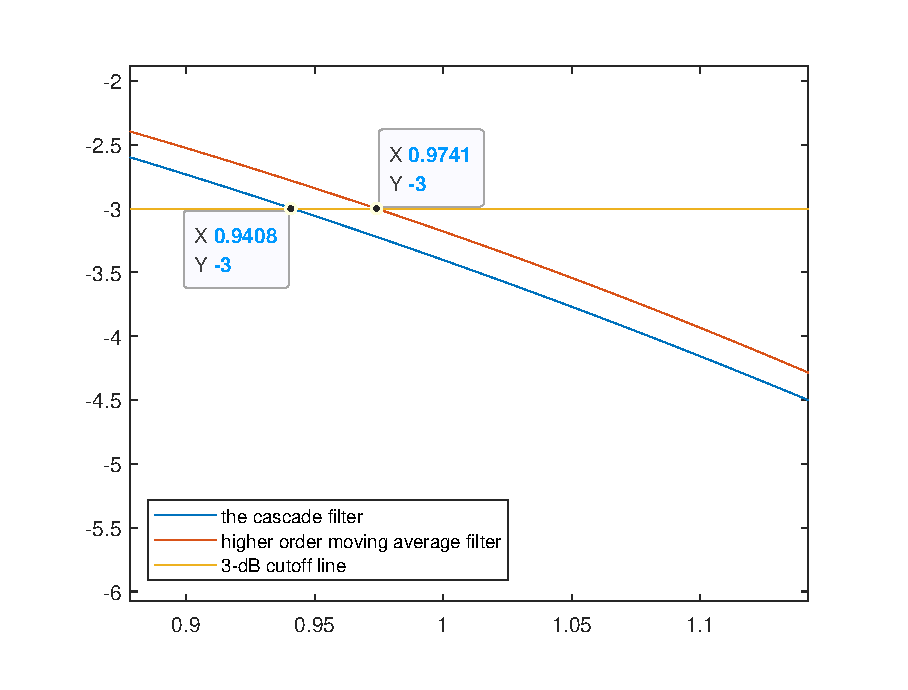
\includegraphics[width=140mm]{pictures/twodesigns2.eps}
    \caption{A tiny look for cutoff frequency}
    \end{figure}
    \item Analysis:\\ 
    Cutoff frequencies for cascade filter and moving average filter are respectively 0.9408(rad) and 0.9471(rad), which approximately equal
    to $0.3\pi$, therefore the design of the two filters are successful.

\end{itemize}
\section*{6.4 IIR Filters}
\addcontentsline{toc}{section}{6.4 IIR Filters}
\begin{info}
\begin{itemize}
    \item In this section, we will design highpass IIR filter with a 3-dB cutoff frequency of 0.2$\pi$.
    \item Compute the 3-dB cutoff frequency for highpass filter:
    Given the first order highpass IIR filter with a zero at $z = 1$:
    $$
    H(z)=\frac{1+\alpha}{2} \frac{1-z^{-1}}{1-\alpha z^{-1}}, \quad 0<|\alpha|<1
    $$
    We could calculate the squared magnitude function:
    $$
    \left|H_{HP}\left(e^{j w}\right)\right|^{2}
    =H\left(e^{j w}\right) H\left(e^{-j w}\right)
    =\frac{(1+\alpha)^{2}(1-c o s w)}{2\left(1+\alpha^{2}-2 \alpha \cos w\right)}
    $$
    \begin{itemize}
        \item Situation 1: Given $\alpha$, calculate $\omega_c$:
        $$
        \frac{(1+\alpha)^{2}(1-c o s w)}{2\left(1+\alpha^{2}-2 \alpha \cos w\right)}=\frac{1}{2}
        $$
        which, when solved, yields:
        $$
        \cos \omega_{c}=\frac{2 \alpha}{1+\alpha^{2}}\ \rightarrow \ \omega_c=\cos^{-1}\frac{2\alpha}{1+\alpha^2}
        $$
        \item  Situation 2: Given $\omega_c$, calculate $\alpha$:
        $$
        \alpha^{2} \cos \omega_c-2 \alpha+\cos \omega_c=0\ \rightarrow \ \alpha=\frac{1-\sqrt{1-\cos^{2} \omega_c}}{\cos \omega_c} 
        $$
        $\therefore$ $\alpha=\frac{1-\sqrt{1-\cos^{2} \omega_c}}{\cos \omega_c}$
    \end{itemize}
    \item In this case, when $\omega_c=0.2\pi$, $\alpha = \frac{1-\sqrt{1-\cos^{2} 0.2\pi}}{\cos 0.2\pi}\approx 0.5095$
\end{itemize}
\end{info}
\begin{itemize}
    \item MATLAB codes in this section:
\end{itemize}
\begin{lstlisting}[title=\textbf{q6\_4.m}]
    clear;
    alpha = (1-sqrt(1-cos(0.2*pi)^2))/cos(0.2*pi);
    w = linspace(0,pi,5000);
    H = sqrt(((1+alpha)^2*(1-cos(w)))./(2*(1+alpha^2-2*alpha*cos(w))));
    plot(w,20*log10(abs(H)));
    hold on;
    plot(w,-3*ones(1,5000));
    xlabel('w(rad)'),ylabel('magnitude response in dB'),title('Simple highpass IIR filter');
    legend('Simple highpass IIR filter','3-dB cutoff line'); 
\end{lstlisting}
\begin{itemize}
    \item Simple highpass IIR filter:
\begin{figure}[H]
\centering
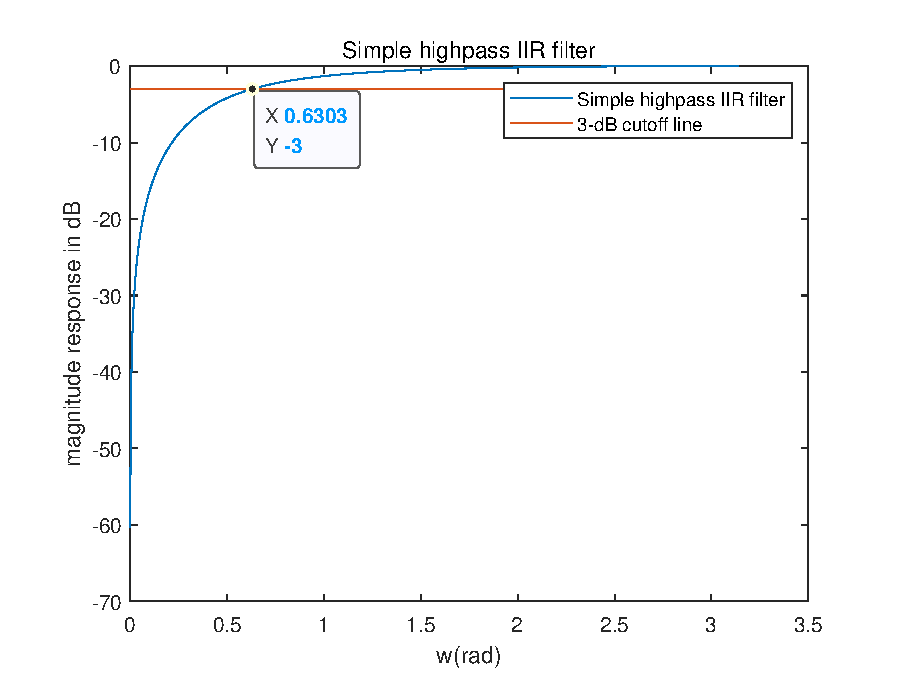
\includegraphics[width=170mm]{pictures/iir.eps}
\caption{Simple highpass IIR filter}
\end{figure}
    \item Analysis:\\
    Resulted cutoff frequency is approximately 0.6303, almost equal to $0.2\pi$. This indicates
    the design of the lowpass filter is successful.
\end{itemize}

\section*{6.5 Summary \& Experience}
\addcontentsline{toc}{section}{6.5 Summary \& Experience}
\begin{enumerate}
    \item In this lab, we mainly completed some specific algorithms of z-transform and some basic designs of linear phase filter and
    IIR filters.
    \item Through this lab, we could easily recover the results both in the labs and lectures, and therefore get a deeper understanding
    of the related knowledge.
    \item Through the designs of some simple filters, the relationship between DTFT and z-transform is emphasized again, which really makes a sense
    to the applications of z-transform. 
\end{enumerate}
\end{document}
